\chapter{Architecture/Model}
\label{cha:architectureAndModel}
This chapter contains the architecture and model of the system, which tools and methods that has been used, how they all connect together to run the experiments and produce the result.
An overview of the system is presented in chapter \ref{sec:overview}. A description of the robot is presented in section \ref{sec:robot}. Section \ref{sec:scenario} contains a description of the different scenarios used in the experiment.

\begin{figure}[h]
\begin{center}
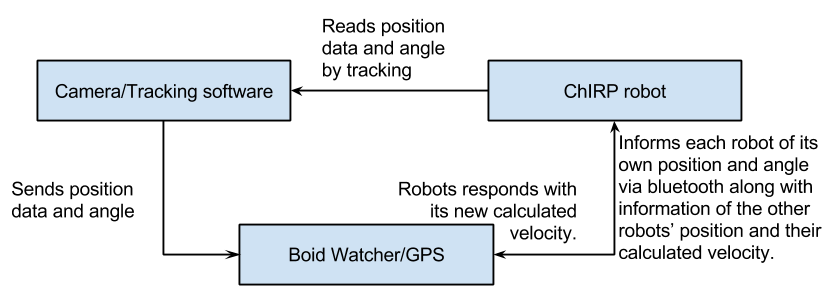
\includegraphics[width=\linewidth]{figs/system_overview}
\end{center}
\caption[System overview]{Overview of the components of the system}
\label{fig:overview}
\end{figure}

\section{System overview}
\label{sec:overview}
The system used in this experiment consists of three primary components as illustrated in figure \ref{fig:overview}: the camera which is used by tracking software, the "Boid-watcher" which is a centralized computer that acts as a GPS and the ChIRP robots.
The camera tracking software tracks each robot's position and its angle, which is sent to the Boid-watcher. The Boid-watcher then forward this information to the robots, it acts as a GPS for the robots. 
The Boid watcher does not only work as a GPS but it is also a bridge between the robots, it provides information about the position and velocity of each robot to all the other robots. The robots can not connect to each other directly, that is why it needs to pass information to other robots via the Boids watcher software.
Even if it is possible for one computer to run both the camera tracking and the watcher software, two different computers were used in this setup. The camera tracking software being run on a stationary desktop computer, and the camera is attached to a pole above a sandbox where the robots roam around. The camera is connected to the stationary desktop. 

The watcher is run on a different computer, in this experiment it was run on a laptop with bluetooth. The watcher software needs to communicate with all the robots simultaneously and that requires processing powers.
The desktop computer was not able to run both the camera tracking software and the watcher software at the same time while sending bluetooth data to all four of the robots. Which lead to the camera not being able to update fast enough and thus crashed quite so often. The bluetooth connection between the computer and the robots might not always be stable, if the connection were to be unstable at times, a reboot of the robot or/and a reconnection of the bluetooth would usually fix the problem.
The camera tracks the robots using image recognition, it recognizes the robots by the two post it notes that are placed on top of each robot. 

%TODO :A simulator created entirely in software were created as well

\section{Robots}
\label{sec:robot}
\begin{figure}
    \centering
    \begin{subfigure}[b]{0.3\textwidth}
        \centering
        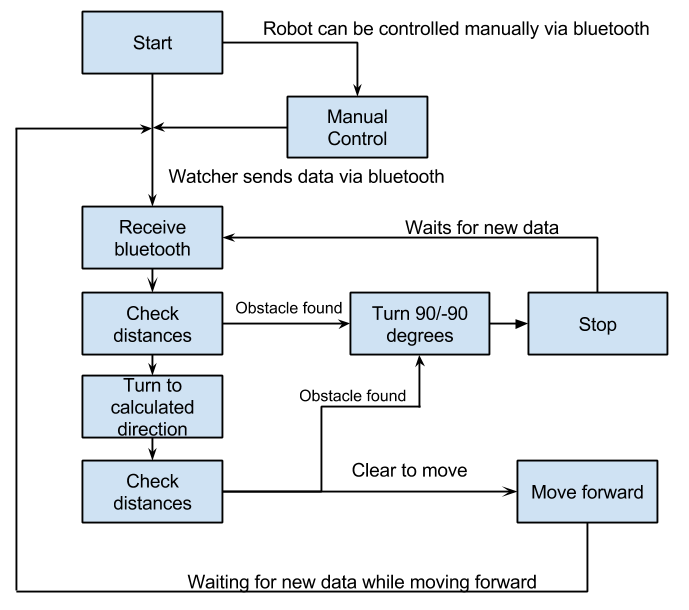
\includegraphics[width=\textwidth]{figs/robotschema.png}
        \caption{$y=x$}
        \label{fig:y equals x}
    \end{subfigure}
    \hfill
    \begin{subfigure}[b]{0.3\textwidth}
        \centering
        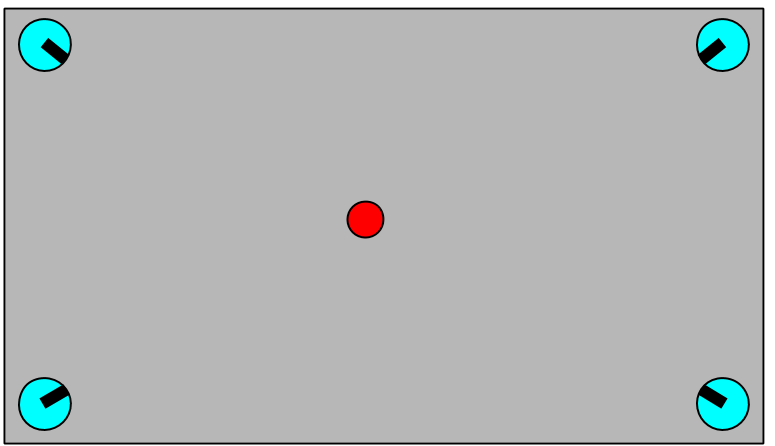
\includegraphics[width=\textwidth]{figs/scenario0.png}
        \caption{$y=3sinx$}
        \label{fig:three sin x}
    \end{subfigure}
    \hfill
    \begin{subfigure}[b]{0.3\textwidth}
        \centering
        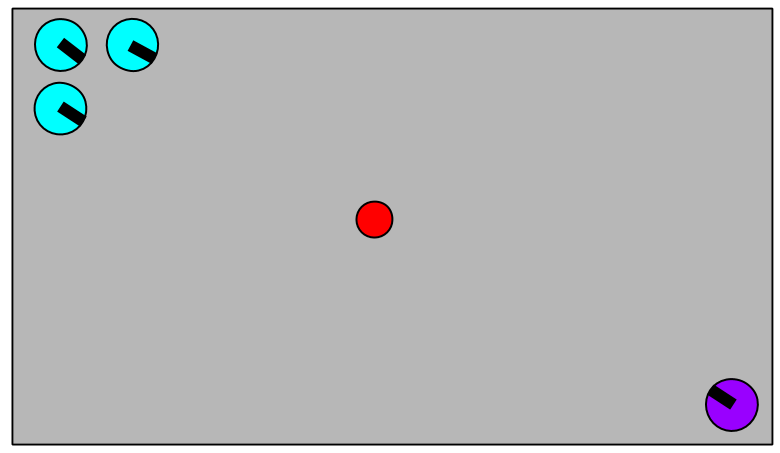
\includegraphics[width=\textwidth]{figs/scenario1.png}
        \caption{$y=5/x$}
        \label{fig:five over x}
    \end{subfigure}
    \caption{Three simple graphs}
    \label{fig:three graphs}
\end{figure}


The robot swarm consist of four ChIRP robots. The ChIRP robot is a circular shaped robot with differential wheel. A differential wheeled robot is a robot with two separate driven wheels on each side, which it can use move itself. If it wants to change its direction it can vary the relative speed of each wheel/motor. For instance if the right wheel moves faster than the left one, the robot will turn to its left.

The advantage of differential wheel is that an additional steering motor is not required for the robot to move around. Usually a caster or additional wheels are added to balance a differential wheeled robot, but the ChIRP robot does not have anything of the sort. Whenever it is moving, the back or the front of the robot is scraping against the floor depending on which way it is moving. This does not affect the movement of the robot.

Each robot is equipped with eight infrared LED lights and receivers used for measuring distance. Infrared light are emitted, reflected of a surface and received in the infrared receiver. For the robot to know how far from an obstacle it is, it measures the amount of infrared it receives. The higher the amount, the closer to the object it is. This holds true for bright or colored surfaces, dark surfaces on the other hand do cause problems because the infrared light is not reflected so well.

The distance sensors are spaced evenly around the robot, where one of the sensors are directly in front of the robot. This sensor can be used to detect whether there is an obstacle directly in front of the robot or not. For this experiment, only the three sensors in front are used. In this experiment the robots should only need to use the three distance sensors in front because the robot only moves forward, so it only needs to determine whether there's an obstacle directly in front of it or not.

Each of the ChIRP robot is equipped with a bluetooth module, which it uses to communicate with the watcher/GPS computer wirelessly. 
The robots are very hollow on top as seen in figure \ref{fig:robot}, and the distance sensors have difficulties sensing other robots due to the hollowness. To counteract the hollowness, a white paper strip was taped around the robots. This makes it easier for the robot to detect the other robots nearby. The same principle was applied to the obstacle used in this experiment. The obstacle is a water bottle filled with water, and a white paper wrapped around it. The water inside the bottle is used to make the bottle heavier, so it does not fall over. And the paper around the bottle is there to reflect the infrared light that the robot uses for measuring distances.

The camera uses image recognition to track the robots. That is why each robot need to have a red and a green post it note on top of it. The red one determines where in the sandbox the robot is located, and the green one is used to determine which way it is pointing. 


\section{Scenarios}
This section explains the setup of each scenario, where each robot is placed in the sandbox, which way it is rotated and where the obstacle is placed. Each scenario have a purpose to demonstrate, which will be explained more in detail.
For this project experiments, three scenarios have been used to generate the results.
\label{sec:scenario}
\begin{figure}[h]
\begin{center}
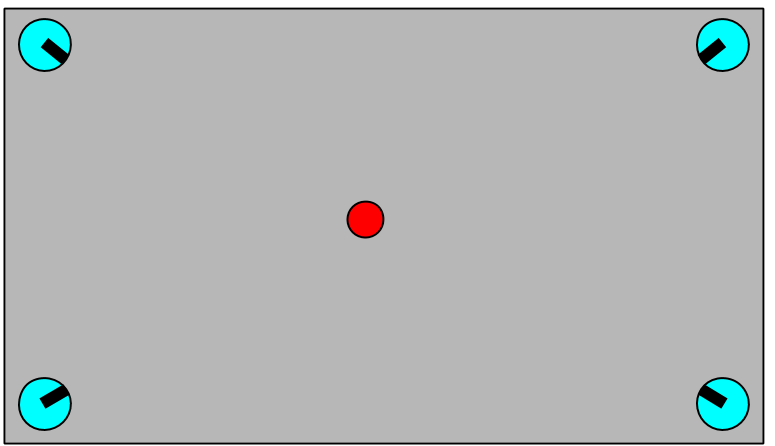
\includegraphics[width=0.8\linewidth]{figs/scenario0}
\end{center}
\caption[scenario 1]{Scenario 1, all the robots are placed in each corner with one obstacle}
\label{fig:scenario0}
\end{figure}

The first scenario is shown in figure \ref{fig:scenario0}, consists of four robots placed on each corner of the sandbox. The reason behind placing each of the robots on each corner of the sandbox is that each robot will be as far from each other as possible. This scenario should demonstrate that the entities are able to flock together, and then stay together as a flock. There is one obstacle placed nearby the middle of the sandbox, the obstacle is placed near the middle to ensure that the robots would encounter it at least once. This scenario would be able to see if the robots actually flocked together like they are supposed to do, and at the same time would be able to avoid the obstacle without bumping or crashing into it.

\begin{figure}[h]
\begin{center}
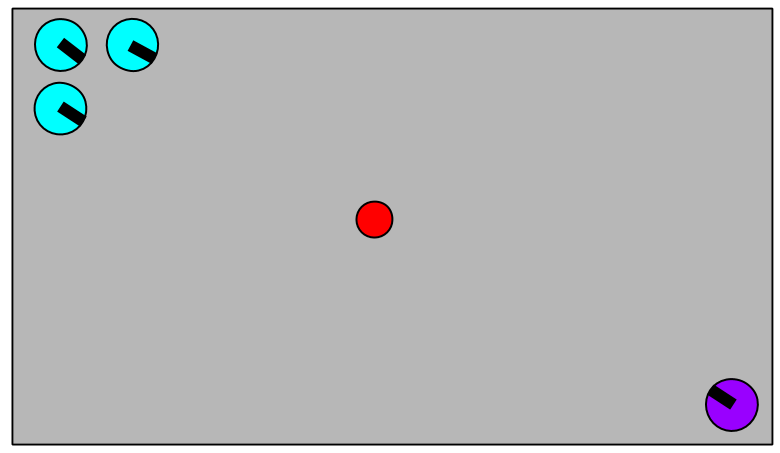
\includegraphics[width=0.8\linewidth]{figs/scenario1}
\end{center}
\caption[scenario 2]{Scenario 2, three robots in one corner, and the last one on the opposite corner}
\label{fig:scenario1}
\end{figure}

The second scenario puts three of entities in one corner, and the last entity is placed on the opposing corner as seen in figure \ref{fig:scenario1}. However the last entity that is placed on the lower right corner by itself will not move, in the case of the physical robot, it will not be turned on. The reason that this entity is a sitting duck placed on the opposite corner of all the other entities is that this robot will act as a goal for the other entities. The obstacle is placed between the lonely robot and the three robots that are clumped up together. The idea behind this setup is that the three robots that start together would try to move to the one that are stationary because they need to flock together. The obstacle in the middle will hinder the robots from moving in a straight line to their goal, which forces them to choose a way around it. 

The third scenario is a scenario where the robots are placed randomly around in the sandbox. The two first scenarios were designed for a specific purpose. The purpose of the third scenario is to demonstrate that the Boids behavior are still intact, even when the robots are placed randomly. The position of the robots, where it should be placed and which way it is pointing was generated randomly by a random number generator. The starting point for this scenario is illustrated in figure \ref{fig:scenario2}.
\begin{figure}[h]
\begin{center}
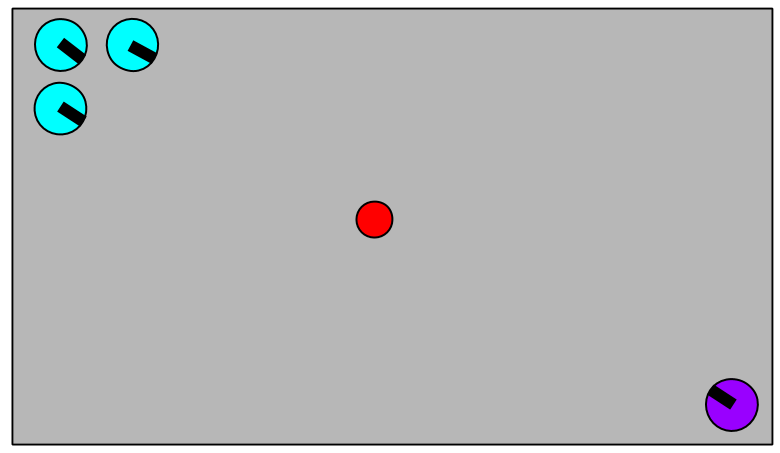
\includegraphics[width=0.8\linewidth]{figs/scenario1}
\end{center}
\caption[scenario 3]{Scenario 3, robots and obstacle randomly placed in the sandbox}
\label{fig:scenario2}
\end{figure}

All the scenarios explained in this thesis used the same sandbox, which is a sandbox with the size of 151.6 cm wide and 123.9 cm long. The only difference between the scenarios are the placement of the robots and the placement of the obstacle. Each scenario were run ten times to generate the data seen in section \ref{sec:results}.
In between each run, the robots had to be placed manually back into their starting position before a new run could take place. To keep the data as consistent as possible, everything else would stay as exactly the same.

\section{Robot controller}
When the robot first is turned on and a bluetooth device is paired with its bluetooth module the robot will stand still and wait. The robot is waiting for a command or data from the watcher software. A human an send command to manually control the robot if needed. If the watcher sends data to the robot, it will start to calculate where it should go based on the data it received. 

When the robot have received all the data it needs to be able to calculate its new direction that it should move to. The robot takes into consideration the position of all the other robots, and their velocity. The position of the other robots are used to determine the sum of the cohesion vector and separation vector. The velocity of the the other robots is used to determine which way they are pointing, and is used to find the alignment vector. A fourth behavior was added for this experiment, which is called the "away from wall" behavior. As the name implies, this is a vector that will lead the robot away from the wall of the sandbox.

, then it will first check the whether there is an obstacle in front of it. %TODO
When the robot has calculated which direction it wants to go, it will find out which direction it needs to face and turn itself approximately in that direction. The robot will then measure the distances once again, in case it has turned towards an obstacle. If there is no obstacle in front of it, it will move forward and wait for new data from the watcher software. If the robot did find an obstacle in front of it, it will turn 90\textdegree to either the right or the left randomly. The robot will stop after turning and wait for new data from the watcher software. 
\begin{figure}[h!]
\begin{center}
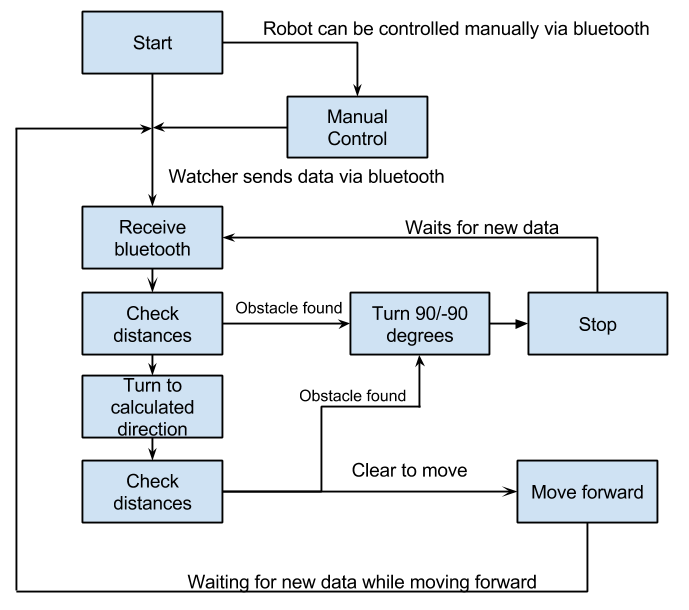
\includegraphics[width=0.8\linewidth]{figs/robotschema}
\end{center}
\caption[Robot flowchart]{Flowchart of the robot}
\label{fig:robotschema}
\end{figure}

\section{Simulator}
A simulator was created where the Boids was implemented solely in software, and rendered on screen, that is no physical robots were used in the simulator. The reason to use a simulator was to see how the Boids were supposed to behave and have a working example to compare with. A typical Boids simulator usually have a wraparound space. If one of the Boids goes outside the window, it will "teleport" to the other side of the window. For example if one of the Boids flies too far to the right and hits the right border, it will loop around and end up on the left side of the screen. That is how the Boids algorithm usually works on a simulator. But physical robots can not loop around the stage like the Boids on the simulator. That is why the simulator used in this project stops the Boids from moving beyond the walls of the window.



\section{Differences between physical and simulator}
The physical robots are trying to mimic the behavior of the Boids created in the simulator. However a physical robot is different than the Boids created in the simulator by nature. As discussed in section \ref{sec:robot}, the robots are a type of differential wheeled robots, which means that it can only move forward or backwards, turn on the spot or move and turn at the same time. The Boids in simulator software did not have any direction, they were able to move freely in all 360\textdegree direction. Which means that if the a Boid in simulator were to move in one direction, it could change its momentum and move the other direct almost instantly. The robot on the other hand would need to turn 180\textdegree before moving forward. The robot is able to reverse its motor to drive backwards, but these Boids robot are not allowed to move backward, and thus have to turn around to move in another direction.

In the simulator, each Boid will know exactly where everything is placed. That is, each Boid knows where all the other Boids are, including itself. It also knows where all the obstacles are. The Boids will have real time access to everything that can be seen on screen. Every Boids will update its perception every frame, that is approximately 60 times every second.

The robots on the other hand, will receive data from the watcher about all the other robots. But due to inaccuracies from the camera and the image processed, the robots only knows vaguely where in the sandbox it is located, and where the others are. The time it takes for a robot to receive new information from the watcher takes roughly one second from the last time it received data from the watcher. If the robots are moving between the time it receives data, it will not know where it is before it receives new data from the watcher software. The camera tracking software are able to see all the robots due to the two post it notes on top, but obstacles found in the sandbox do not contain any color or anything that the camera can track. Obstacles are therefore ignored by the camera tracker software because it does not support tracking of anything other than the robots. That is why the robots needs to use their distance sensors in front to detect the obstacles.

The biggest difference between the physical experiment in the sandbox and the simulated Boids is the size and speed of the entities. The size of the simulator is 1024 px times 1024 px. While the sandbox is 151.6 cm wide and 123.9 cm long, which is 800x652 px in the watcher software.

